
\section{GAT-Denoiser}

\begin{frame}{GAT-Denoiser}
  \begin{itemize}
    \item GAT-Denoiser is a graph neural network (GNN) to denoise observations.
    \item Consists of three components:
    \begin{itemize}
      \item Convolution
      \item Graph Attention Network (GAT) \cite{GAT}
      \item End-to-End Learning
    \end{itemize}
  \end{itemize}

  \only<2>{
    \begin{figure}
      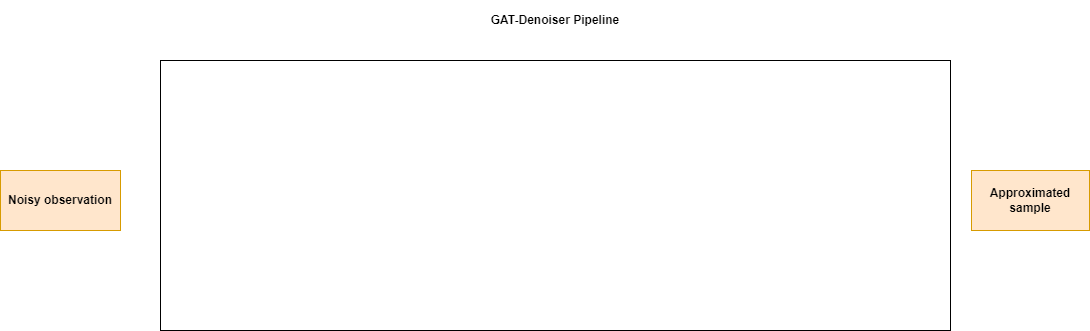
\includegraphics[width=\textwidth]{Overall_GAT-Denoiser_Pipeline_3.drawio.png}
    \end{figure}
  }

  \only<3>{
    \begin{figure}
      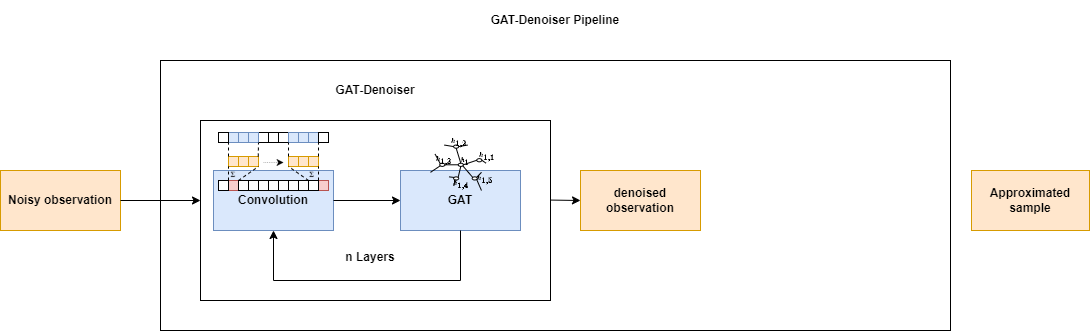
\includegraphics[width=\textwidth]{Overall_GAT-Denoiser_Pipeline_2.drawio.png}
    \end{figure}
  }

  \only<4>{
    \begin{figure}
      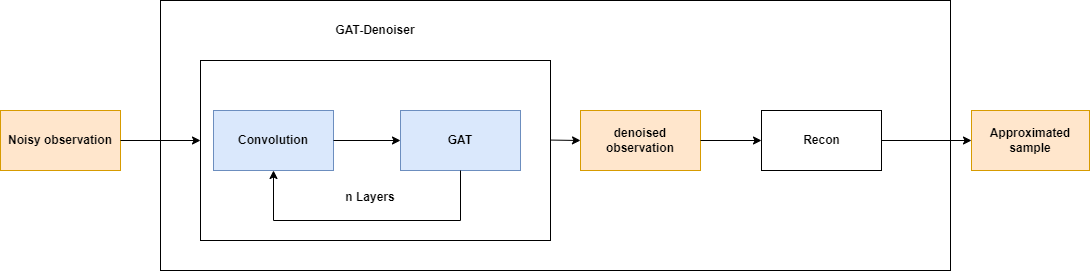
\includegraphics[width=\textwidth]{Overall_GAT-Denoiser_Pipeline.drawio.png}
    \end{figure}
  }

\end{frame}

\begin{frame}{GAT-Denoiser Components}
    
  \begin{itemize}
    \item<2-> Convolution
    \begin{itemize}
      \item Denoise single observation
    \end{itemize}

    \item<3-> Graph Attention Network (GAT) \cite{GAT}
    \begin{itemize}
      \item Denoise neighboring  observation
    \end{itemize}
    \item<4-> End-to-End Learning
    \begin{itemize}
      \item Optimize for reconstruction quality
      \item $\mathcal{L} &= \parallel x - \textit{Recon} ( \textit{GAT-Denoiser}(A(x, \theta) + \eta)) \parallel ^2_2$
      \item $\mathcal{L}_{sino} &= \parallel p - \textit{GAT-Denoiser}(A(x, \theta) + \eta) \parallel ^2_2 $
    \end{itemize}
  \end{itemize}

\end{frame}

\begin{frame}{Graph Attention Network - GAT}
  \begin{columns}
  \column{0.6\textwidth}
    \begin{itemize}
      \item Extends Graph Convolution Network with attention (weights)
      \item Compute new node features
      \item Averages graph over neighborhood
      \item Multi-head available, motivated by \cite{transformer}
      \item<2> \alert<2>{$\sigma$: activation function (Exponential Linear Unit)}
      \item<2> \alert<2>{$W$: learnable weight matrix}
      \item<2> \alert<2>{$\alpha$: normalized attention coefficients}
    \end{itemize}
    \column{0.4\textwidth}
    \begin{figure}
      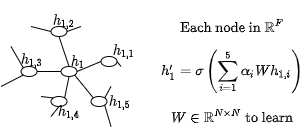
\includegraphics[width=.6\textwidth]{GAT.drawio.png}
    \end{figure}
    \only<2>{
      $$h_{1}^{\prime} = \sigma \left( \sum_{i=1}^5\alpha_i W h_{1,i} \right)$$
    }
    
  \end{columns}

\end{frame}


\begin{frame}{Input Graph}
  \pause
  \begin{columns}
    \column{0.6\textwidth}
    \begin{itemize}
      \item Exploit information from GL
      \item Low-dimensional embedding estimates angles
      \item Dominant information in data can be considered observation angles.
      \item<3-> \alert<3>{Construct graph from observation angles}
    \end{itemize}
    \column{0.4\textwidth}

    \only<4>{
      \begin{figure}
        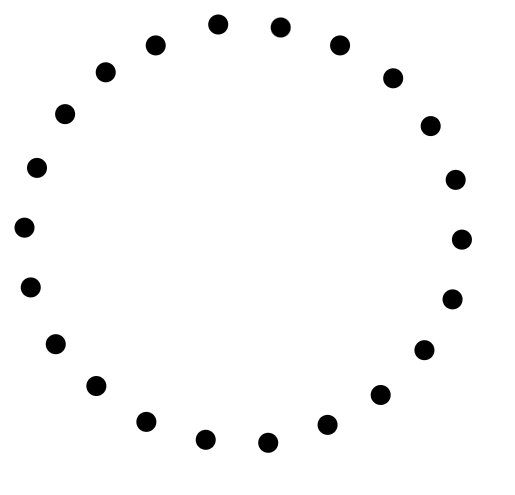
\includegraphics[width=.7\textwidth]{Circle_graph.drawio.png}
      \end{figure}
    }

    \only<5-6>{
      \begin{figure}
        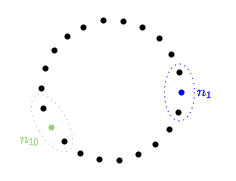
\includegraphics[width=.85\textwidth]{Circle_graphneighbours.drawio.png}
      \end{figure}
    }
    
  \end{columns}
  

  \begin{tcolorbox}[colback=red!5!white,hide=<1-4>, alert=<5>, colframe=red!75!black]
    Observation angles  $\theta$ are assumed to be equally spaced.
\end{tcolorbox}
\end{frame}


\begin{frame}{GAT-Denoiser Implementation for Computed Tomography}
  \begin{itemize}
    \item Use U-Net for reconstruction
    \item During Trainig, U-Net might be trained jointly
  \end{itemize}
\end{frame}

